\begin{exercises}
\textit{In problems 1--4, graph the solution set for each linear inequality.}\\
\ptwo{
\[3x+y < 4\]
\begin{center}
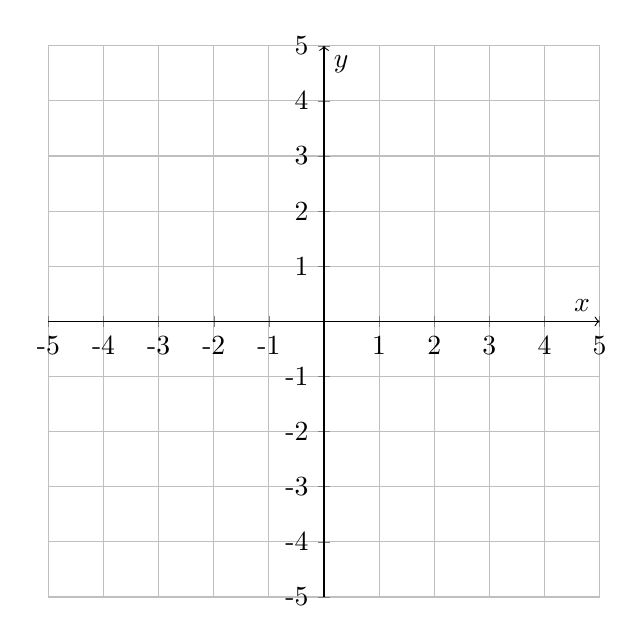
\begin{tikzpicture}
\begin{axis}[
    xmin=-5, xmax=5,
    ymin=-5, ymax=5,
    axis lines=center,
    axis on top=false,
    domain=0:1,
    x=0.7cm,
    y=0.7cm,
    xtick={-10,-9,...,10},
    xticklabels={-10,-9,...,10},
    ytick={-10,-9,...,10},
    yticklabels={-10,-9,...,10},
    axis lines=middle,
    axis line style={->},
    xlabel={$x$},
    ylabel={$y$},
    grid=major
    ]
    
\end{axis}
\end{tikzpicture}
\end{center}}
\ptwo{
\[x \geq y-2\]
\begin{center}
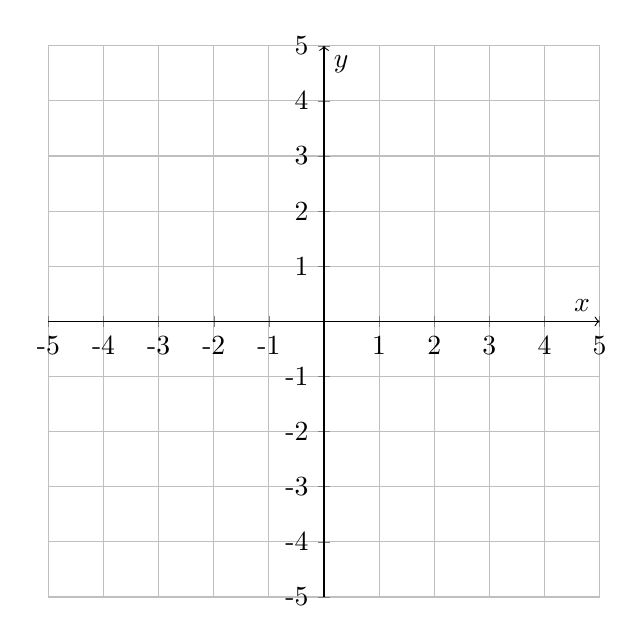
\begin{tikzpicture}
\begin{axis}[
    xmin=-5, xmax=5,
    ymin=-5, ymax=5,
    axis lines=center,
    axis on top=false,
    domain=0:1,
    x=0.7cm,
    y=0.7cm,
    xtick={-10,-9,...,10},
    xticklabels={-10,-9,...,10},
    ytick={-10,-9,...,10},
    yticklabels={-10,-9,...,10},
    axis lines=middle,
    axis line style={->},
    xlabel={$x$},
    ylabel={$y$},
    grid=major
    ]
    
\end{axis}
\end{tikzpicture}
\end{center}}

\ptwo{
\[2x-2y > 4\]
\begin{center}
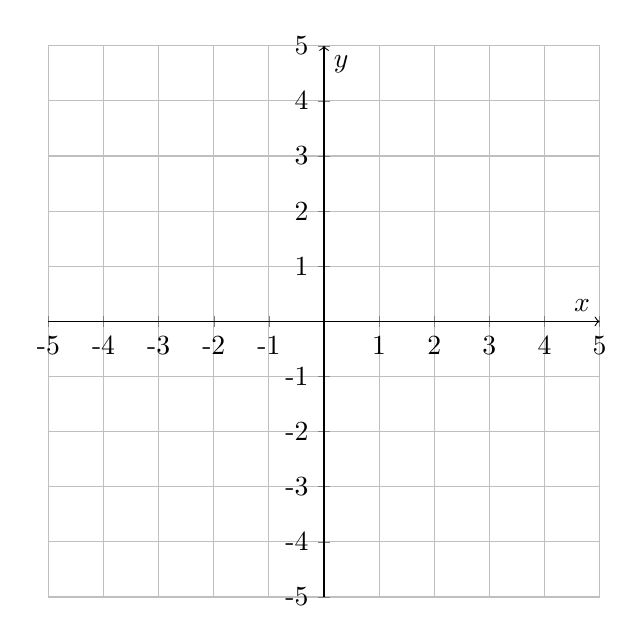
\begin{tikzpicture}
\begin{axis}[
    xmin=-5, xmax=5,
    ymin=-5, ymax=5,
    axis lines=center,
    axis on top=false,
    domain=0:1,
    x=0.7cm,
    y=0.7cm,
    xtick={-10,-9,...,10},
    xticklabels={-10,-9,...,10},
    ytick={-10,-9,...,10},
    yticklabels={-10,-9,...,10},
    axis lines=middle,
    axis line style={->},
    xlabel={$x$},
    ylabel={$y$},
    grid=major
    ]
    
\end{axis}
\end{tikzpicture}
\end{center}}
\ptwo{
\[y \leq \dfrac{1}{2}x-1\]
\begin{center}
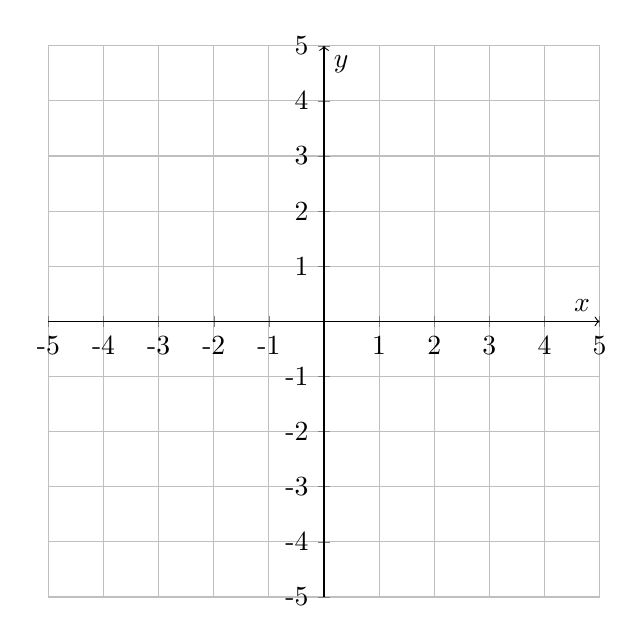
\begin{tikzpicture}
\begin{axis}[
    xmin=-5, xmax=5,
    ymin=-5, ymax=5,
    axis lines=center,
    axis on top=false,
    domain=0:1,
    x=0.7cm,
    y=0.7cm,
    xtick={-10,-9,...,10},
    xticklabels={-10,-9,...,10},
    ytick={-10,-9,...,10},
    yticklabels={-10,-9,...,10},
    axis lines=middle,
    axis line style={->},
    xlabel={$x$},
    ylabel={$y$},
    grid=major
    ]
    
\end{axis}
\end{tikzpicture}
\end{center}}
\vfill
\pagebreak

\textit{In problems 5--12, graph the solution set for each system of inequalities.}\\
\ptwo{
\begin{align*}
x-3y &> -6\\
x &\leq -3
\end{align*}
\begin{center}
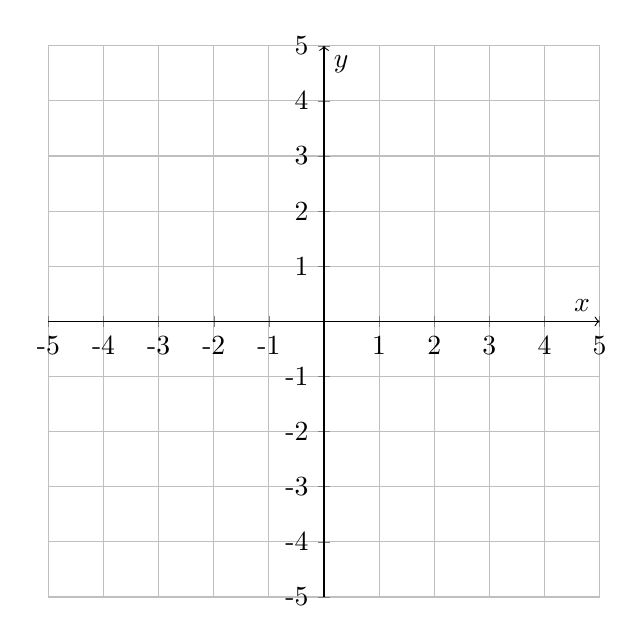
\begin{tikzpicture}
\begin{axis}[
    xmin=-5, xmax=5,
    ymin=-5, ymax=5,
    axis lines=center,
    axis on top=false,
    domain=0:1,
    x=0.7cm,
    y=0.7cm,
    xtick={-10,-9,...,10},
    xticklabels={-10,-9,...,10},
    ytick={-10,-9,...,10},
    yticklabels={-10,-9,...,10},
    axis lines=middle,
    axis line style={->},
    xlabel={$x$},
    ylabel={$y$},
    grid=major
    ]
    
\end{axis}
\end{tikzpicture}
\end{center}}
\ptwo{
\begin{align*}
3x+4y &< 12\\
y &\geq -2x+1
\end{align*}
\begin{center}
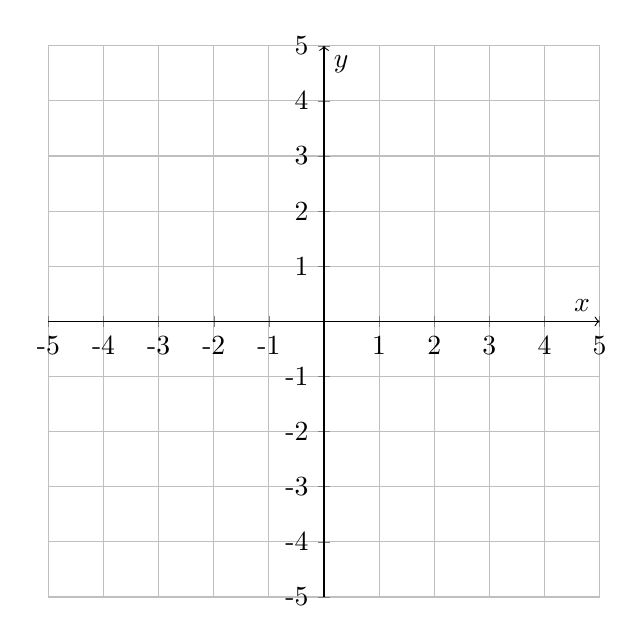
\begin{tikzpicture}
\begin{axis}[
    xmin=-5, xmax=5,
    ymin=-5, ymax=5,
    axis lines=center,
    axis on top=false,
    domain=0:1,
    x=0.7cm,
    y=0.7cm,
    xtick={-10,-9,...,10},
    xticklabels={-10,-9,...,10},
    ytick={-10,-9,...,10},
    yticklabels={-10,-9,...,10},
    axis lines=middle,
    axis line style={->},
    xlabel={$x$},
    ylabel={$y$},
    grid=major
    ]
    
\end{axis}
\end{tikzpicture}
\end{center}}

\ptwo{
\begin{align*}
x &\geq y-3\\
y &> 2x+1
\end{align*}
\begin{center}
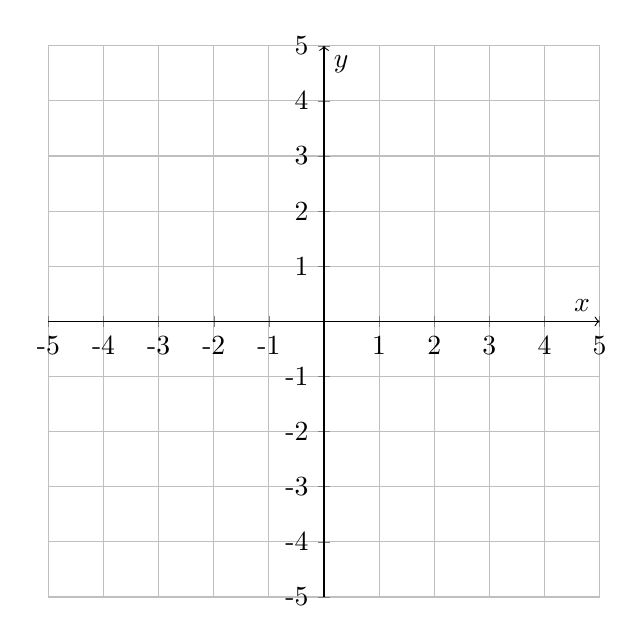
\begin{tikzpicture}
\begin{axis}[
    xmin=-5, xmax=5,
    ymin=-5, ymax=5,
    axis lines=center,
    axis on top=false,
    domain=0:1,
    x=0.7cm,
    y=0.7cm,
    xtick={-10,-9,...,10},
    xticklabels={-10,-9,...,10},
    ytick={-10,-9,...,10},
    yticklabels={-10,-9,...,10},
    axis lines=middle,
    axis line style={->},
    xlabel={$x$},
    ylabel={$y$},
    grid=major
    ]
    
\end{axis}
\end{tikzpicture}
\end{center}}
\ptwo{
\begin{align*}
y &> -4\\
x &\leq 2
\end{align*}
\begin{center}
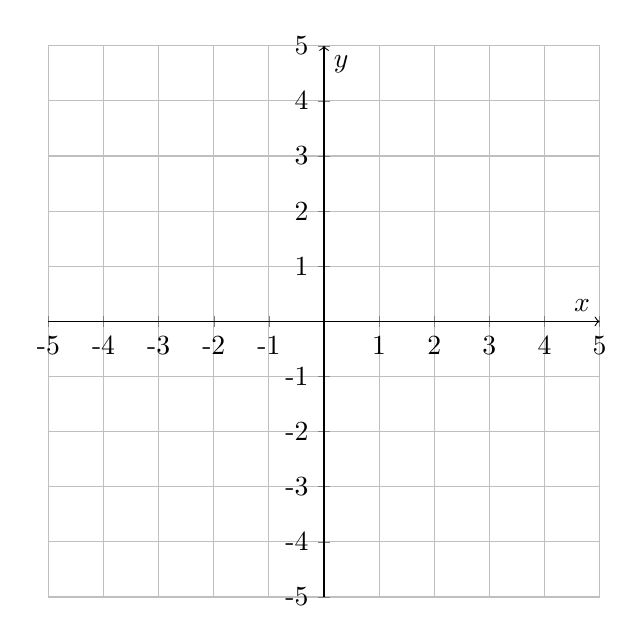
\begin{tikzpicture}
\begin{axis}[
    xmin=-5, xmax=5,
    ymin=-5, ymax=5,
    axis lines=center,
    axis on top=false,
    domain=0:1,
    x=0.7cm,
    y=0.7cm,
    xtick={-10,-9,...,10},
    xticklabels={-10,-9,...,10},
    ytick={-10,-9,...,10},
    yticklabels={-10,-9,...,10},
    axis lines=middle,
    axis line style={->},
    xlabel={$x$},
    ylabel={$y$},
    grid=major
    ]
    
\end{axis}
\end{tikzpicture}
\end{center}}
\vfill
\pagebreak

\ptwo{
\begin{align*}
x+y &> -4\\
x-y &\leq 0
\end{align*}
\begin{center}
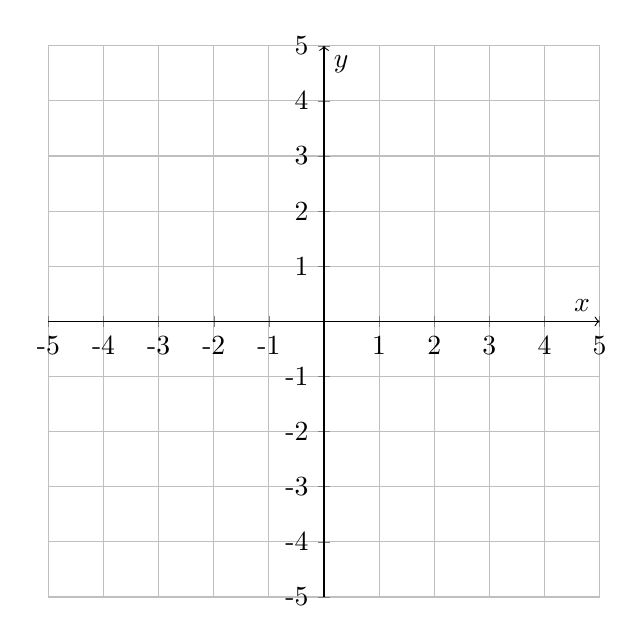
\begin{tikzpicture}
\begin{axis}[
    xmin=-5, xmax=5,
    ymin=-5, ymax=5,
    axis lines=center,
    axis on top=false,
    domain=0:1,
    x=0.7cm,
    y=0.7cm,
    xtick={-10,-9,...,10},
    xticklabels={-10,-9,...,10},
    ytick={-10,-9,...,10},
    yticklabels={-10,-9,...,10},
    axis lines=middle,
    axis line style={->},
    xlabel={$x$},
    ylabel={$y$},
    grid=major
    ]
    
\end{axis}
\end{tikzpicture}
\end{center}}
\ptwo{
\begin{align*}
2x-5y &\leq -10\\
y &< 3
\end{align*}
\begin{center}
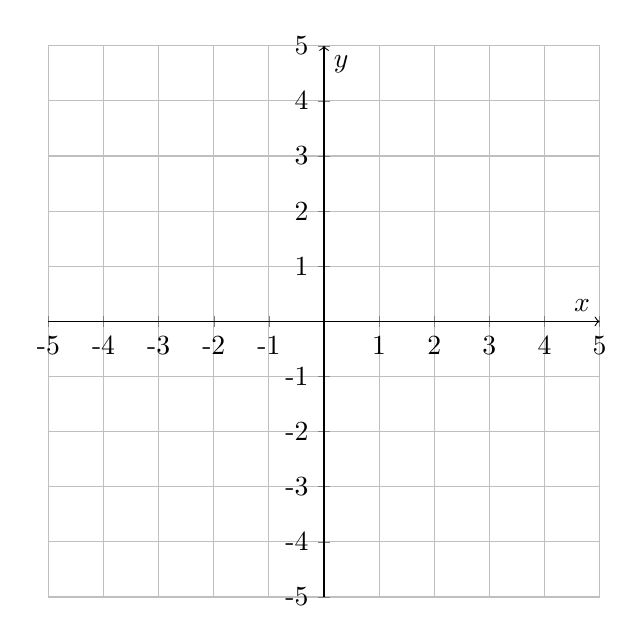
\begin{tikzpicture}
\begin{axis}[
    xmin=-5, xmax=5,
    ymin=-5, ymax=5,
    axis lines=center,
    axis on top=false,
    domain=0:1,
    x=0.7cm,
    y=0.7cm,
    xtick={-10,-9,...,10},
    xticklabels={-10,-9,...,10},
    ytick={-10,-9,...,10},
    yticklabels={-10,-9,...,10},
    axis lines=middle,
    axis line style={->},
    xlabel={$x$},
    ylabel={$y$},
    grid=major
    ]
    
\end{axis}
\end{tikzpicture}
\end{center}}

\ptwo{
\begin{align*}
4x+5y &< 20\\
y &> -\dfrac{1}{3}x+2
\end{align*}
\begin{center}
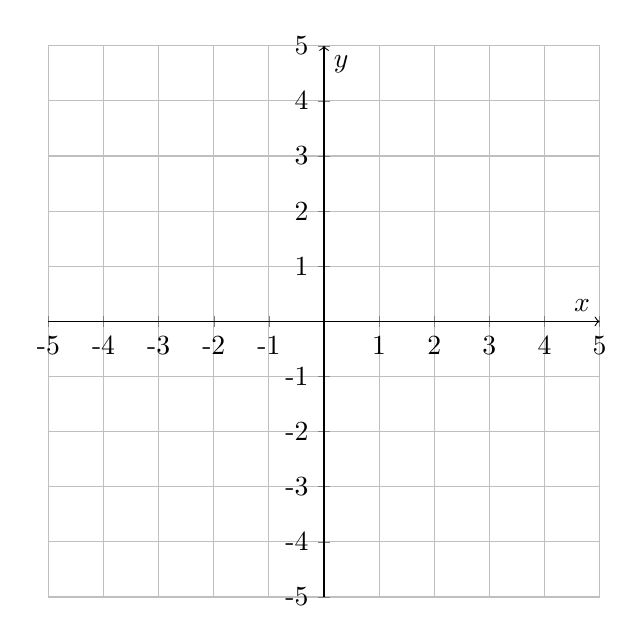
\begin{tikzpicture}
\begin{axis}[
    xmin=-5, xmax=5,
    ymin=-5, ymax=5,
    axis lines=center,
    axis on top=false,
    domain=0:1,
    x=0.7cm,
    y=0.7cm,
    xtick={-10,-9,...,10},
    xticklabels={-10,-9,...,10},
    ytick={-10,-9,...,10},
    yticklabels={-10,-9,...,10},
    axis lines=middle,
    axis line style={->},
    xlabel={$x$},
    ylabel={$y$},
    grid=major
    ]
    
\end{axis}
\end{tikzpicture}
\end{center}}
\ptwo{
\begin{align*}
y &> \dfrac{3}{5}x-4\\
y &\leq -\dfrac{4}{3}x+3
\end{align*}
\begin{center}
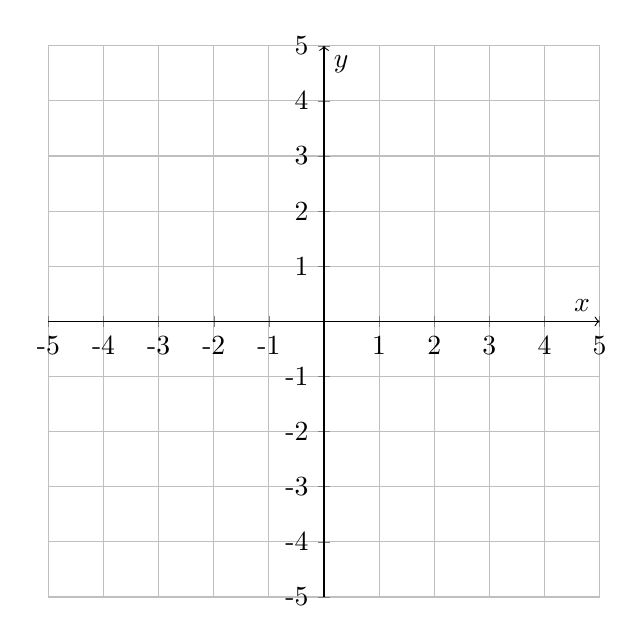
\begin{tikzpicture}
\begin{axis}[
    xmin=-5, xmax=5,
    ymin=-5, ymax=5,
    axis lines=center,
    axis on top=false,
    domain=0:1,
    x=0.7cm,
    y=0.7cm,
    xtick={-10,-9,...,10},
    xticklabels={-10,-9,...,10},
    ytick={-10,-9,...,10},
    yticklabels={-10,-9,...,10},
    axis lines=middle,
    axis line style={->},
    xlabel={$x$},
    ylabel={$y$},
    grid=major
    ]
    
\end{axis}
\end{tikzpicture}
\end{center}}
\end{exercises}